% Original teaching adaptation of Heather Macbeth, The Mechanics of Proof, Chapter 9.
% Source: https://hrmacbeth.github.io/math2001/09_Sets.html
% Source repository: hrmacbeth/math2001, e660f42b13ddcb6d12b52ba036d6bd071a0cfb9b.
% All prose and diagrams are newly written. Lean demonstrations are not build-verified.
% CSC302 lecture slides adapted from Heather Macbeth, The Mechanics of Proof.
\documentclass[aspectratio=169,11pt]{beamer}
\usepackage[T1]{fontenc}
\usepackage{lmodern}
\usepackage{amsmath,amssymb,mathtools}
\usepackage{booktabs,array,listings,tikz}
\usetikzlibrary{arrows.meta,positioning,calc}
\definecolor{ProofNavy}{HTML}{18324F}
\definecolor{ProofTeal}{HTML}{007D82}
\definecolor{ProofPaper}{HTML}{F3F6F8}
\usetheme{default}
\setbeamercolor{normal text}{fg=ProofNavy,bg=white}
\setbeamercolor{structure}{fg=ProofTeal}
\setbeamercolor{frametitle}{fg=ProofNavy}
\setbeamercolor{block title}{fg=white,bg=ProofNavy}
\setbeamercolor{block body}{fg=ProofNavy,bg=ProofPaper}
\setbeamercolor{block title example}{fg=white,bg=ProofTeal}
\setbeamercolor{block body example}{fg=ProofNavy,bg=ProofPaper}
\setbeamerfont{frametitle}{size=\Large,series=\bfseries}
\setbeamertemplate{navigation symbols}{}
\setbeamertemplate{itemize item}{\small\textbullet}
\setbeamertemplate{footline}{%
  \leavevmode\hbox{%
  \begin{beamercolorbox}[wd=.86\paperwidth,ht=2.8ex,dp=1.2ex,leftskip=1.6em]{author in head/foot}%
    \scriptsize CSC302\quad\textbar\quad\insertshorttitle
  \end{beamercolorbox}%
  \begin{beamercolorbox}[wd=.14\paperwidth,ht=2.8ex,dp=1.2ex,rightskip=1.6em plus1fil]{date in head/foot}%
    \scriptsize\insertframenumber/\inserttotalframenumber
  \end{beamercolorbox}}}
\setbeamersize{text margin left=8mm,text margin right=8mm}
\lstdefinelanguage{Lean}{%
  morekeywords={example,theorem,lemma,def,by,calc,have,exact,apply,intro,intros,constructor,rcases,rfl,rw,ring,numbers,linarith,nlinarith,rel,extra,addarith,obtain,left,right,use,choose,dsimp,change,ext,fun,show,from,at,with,induction,case,decide,contradiction,push_neg,by_cases,by_contra,assumption,existsi,simp,simpa},
  sensitive=true,morecomment=[l]{--},morestring=[b]"}
\lstset{language=Lean,basicstyle=\ttfamily\small,keywordstyle=\color{ProofTeal}\bfseries,
  commentstyle=\color{gray},stringstyle=\color{ProofNavy},showstringspaces=false,
  columns=fullflexible,keepspaces=true,breaklines=true,frame=single,
  rulecolor=\color{ProofTeal!30},backgroundcolor=\color{ProofPaper},
  aboveskip=0.5em,belowskip=0.4em}
\newcommand{\N}{\mathbb{N}}
\newcommand{\Z}{\mathbb{Z}}
\newcommand{\Q}{\mathbb{Q}}
\newcommand{\R}{\mathbb{R}}
\newcommand{\coursechapter}[2]{%
  \title[Chapter #1: #2]{Chapter #1\\#2}%
  \subtitle{The Mechanics of Proof \textbar{} CSC302 lecture notes}%
  \author{Based on Heather Macbeth's textbook}%
  \date{}%
}
\newcommand{\sourcecredit}[1]{\par\vfill{\tiny Source: Heather Macbeth, \emph{The Mechanics of Proof}, #1.}}
\newcommand{\bookurl}{\url{https://hrmacbeth.github.io/math2001/}}
\hypersetup{colorlinks=true,urlcolor=ProofTeal,linkcolor=ProofNavy}

\coursechapter{9}{Sets}
\begin{document}
\begin{frame}
\titlepage
\end{frame}

% Source: Chapter 9 introduction and Definitions 9.1.1, 9.3.1.
\begin{frame}{What we will learn}
\begin{itemize}
\item Translate membership, inclusion, and equality into logical statements.
\item Prove statements about unions, intersections, and complements.
\item Keep the ambient type explicit, including for empty and universal sets.
\item Treat sets as inputs and outputs of functions.
\item Prove that no function $X\to\mathcal P(X)$ can be surjective.
\end{itemize}
\begin{block}{The organizing idea}
A set in a type $X$ is specified by a predicate on $X$.
To ask whether $x$ belongs to the set is to ask whether that predicate holds at $x$.
\end{block}
\sourcecredit{Chapter 9; Sections 9.1--9.3}
\end{frame}

\section{9.1 Introduction}
% Source: Examples 9.1.1--9.1.2.
\begin{frame}{9.1: Membership evaluates a predicate}
For a predicate $P$ on $X$, write
\[
 S=\{x:X\mid P(x)\},\qquad a\in S\ \Longleftrightarrow\ P(a).
\]
The notation $a\notin S$ means $\neg(a\in S)$.
\begin{exampleblock}{A concrete set of integers}
Let $S=\{n:\Z\mid n\le3\}$.
Then $1\in S$ because $1\le3$, while $7\notin S$ because $7\nleq3$.
Negative integers can also belong to $S$: for example, $-10\le3$.
\end{exampleblock}
\begin{exampleblock}{A set defined by parity}
For $O=\{n:\N\mid n\text{ is odd}\}$, we have $10\notin O$:
$10=2\cdot5$ is even, and no natural number is both even and odd.
\end{exampleblock}
\sourcecredit{Examples 9.1.1--9.1.2}
\end{frame}

% Source: Definition and example 9.1.3.
% Correction: the prose display a=4a is a typo; the witness equation is a=4k.
\begin{frame}{Inclusion is a universal implication}
\begin{block}{Definition}
For sets $U,V$ in the same type $X$,
\[
 U\subseteq V\quad\Longleftrightarrow\quad
 \forall x\in X,\quad x\in U\ \Longrightarrow\ x\in V.
\]
\end{block}
\textbf{Claim.} $\{a:\N\mid4\mid a\}\subseteq\{b:\N\mid2\mid b\}$.
\medskip

\textbf{Proof.} Choose an arbitrary $a\in\N$ with $4\mid a$.
There is a $k\in\N$ with $a=4k$. Now
\[
 a=4k=2(2k).
\]
The witness $2k\in\N$ proves $2\mid a$. Therefore every element of the first set
belongs to the second.
\sourcecredit{Example 9.1.3}
\end{frame}

% Source: Examples 9.1.4 and 9.1.6; witnesses and derivations newly phrased.
\begin{frame}{To refute inclusion, find an element that escapes}
\[
 U\not\subseteq V\quad\Longleftrightarrow\quad
 \exists x\in X,\quad x\in U\ \land\ x\notin V.
\]
For $U=\{x:\R\mid0\le x^2\}$ and $V=\{x:\R\mid0\le x\}$,
the witness $x=-3$ works: $0\le(-3)^2=9$, but $-3<0$.
\medskip

An element in just one of two sets also proves the sets unequal.
For example,
\[
 \{n:\N\mid4\mid n\}\ne\{n:\N\mid2\mid n\}.
\]
Indeed, $6=2\cdot3$, so $6$ belongs to the second set.
If $6=4k$ with $k\in\N$, then either $k\le1$ gives $4k\le4$, or $k\ge2$ gives
$4k\ge8$. Thus $6$ is absent from the first set.
\sourcecredit{Examples 9.1.4 and 9.1.6}
\end{frame}

% Source: Example 9.1.5, same integer witness translations.
\begin{frame}{Set equality means the same membership test}
\begin{block}{Extensionality}
$U=V$ if and only if $\forall x\in X,\ x\in U\iff x\in V$.
Equivalently, prove both $U\subseteq V$ and $V\subseteq U$.
\end{block}
\textbf{Example.} The sets
\[
 O=\{x:\Z\mid x\text{ is odd}\},\qquad
 M=\{x:\Z\mid\exists k\in\Z,\ x=2k-1\}
\]
are equal. Fix $x\in\Z$.
\begin{itemize}
\item If $x\in O$, write $x=2l+1=2(l+1)-1$. The integer witness $k=l+1$ gives $x\in M$.
\item If $x\in M$, write $x=2k-1=2(k-1)+1$. The integer witness $l=k-1$ shows that $x$ is odd.
\end{itemize}
Both implications hold for every $x$, hence $O=M$.
\sourcecredit{Example 9.1.5}
\end{frame}

% Source: Example 9.1.8; factorization and two converse cases are retained.
\begin{frame}{Finite sets turn membership into alternatives}
For a fixed ambient type,
\[
 x\in\{a,b\}\quad\Longleftrightarrow\quad x=a\ \lor\ x=b.
\]
Order and repetitions do not affect a set: $\{a,b,a\}=\{b,a\}$.
\begin{exampleblock}{A complete solution set}
We claim $\{x:\R\mid x^2-x-2=0\}=\{-1,2\}$.
For an arbitrary real $x$:
\begin{itemize}
\item If $x^2-x-2=0$, then $(x+1)(x-2)=0$.
Since $\R$ has no zero divisors, $x+1=0$ or $x-2=0$, giving $x=-1$ or $x=2$.
\item Conversely, substituting $x=-1$ gives $1+1-2=0$;
substituting $x=2$ gives $4-2-2=0$.
\end{itemize}
\end{exampleblock}
\sourcecredit{Example 9.1.8}
\end{frame}

% Source: Example 9.1.3, with divisibility unfolded to an ASCII Exists predicate.
\begin{frame}[fragile]{Lean: Strip off the set notation}
\begin{lstlisting}
example : Set.Subset
    {a : Nat | Exists (fun k : Nat => a = 4 * k)}
    {b : Nat | Exists (fun j : Nat => b = 2 * j)} := by
  intro a ha
  cases ha with
  | intro k hk =>
      use 2 * k
      calc a = 4 * k := hk
        _ = 2 * (2 * k) := by ring
\end{lstlisting}
Here \texttt{Exists} spells out the divisibility witness.
\begin{center}
\begin{tabular}{ll}
Membership & \texttt{dsimp} exposes the predicate.\\
Subset & \texttt{intro x hx} starts the implication.\\
Set equality & \texttt{ext x} creates a membership equivalence.
\end{tabular}
\end{center}
\sourcecredit{Examples 9.1.1, 9.1.3, and 9.1.5; textbook-environment demonstration}
\end{frame}

% Source: Exercises 9.1.10, inclusion of multiples and incomplete root set.
\begin{frame}{Practice 9.1: Do the sets contain exactly what is claimed?}
\begin{enumerate}
\item Prove $\{n:\N\mid20\mid n\}\subseteq\{n:\N\mid5\mid n\}$.
Is the reverse inclusion true?
\item Prove or disprove
\[
 \{t:\R\mid t^2-5t+4=0\}=\{4\}.
\]
\item Decide whether $-3$ belongs to
$\{x:\R\mid\forall y\in\R,\ x\le y^2\}$.
\end{enumerate}
State the logical form of each task before proving it.
An equation satisfied by every listed element does not prove the list is complete.
\sourcecredit{Exercises 9.1.10}
\end{frame}

% Source: Newly written solutions to Exercises 9.1.10.
\begin{frame}{Practice 9.1: Solution ideas}
\begin{enumerate}
\item If $n=20k$, then $n=5(4k)$, so $5\mid n$.
The reverse inclusion fails at $n=5$: it is a multiple of $5$ but not of $20$.
\item The equality is false. The witness $t=1$ satisfies $1-5+4=0$,
but $1\notin\{4\}$. In fact,
$(t-1)(t-4)=t^2-5t+4$, so the full solution set is $\{1,4\}$.
\item Yes. For every real $y$, $y^2\ge0$, hence $-3\le0\le y^2$.
The same input $-3$ works for \emph{all} values quantified inside the predicate.
\end{enumerate}
\sourcecredit{Exercises 9.1.10}
\end{frame}

\section{9.2 Set operations}
% Source: Definitions in Examples 9.2.1, 9.2.3, 9.2.5--9.2.7.
\begin{frame}{9.2: Set operations package familiar logical operations}
Fix sets $U,V$ in a type $X$ and an element $x\in X$.
\begin{center}
\begin{tabular}{lll}
\toprule
Set & Membership condition & Logical operation\\\midrule
$U\cup V$ & $x\in U\lor x\in V$ & or\\
$U\cap V$ & $x\in U\land x\in V$ & and\\
$U^c$ & $x\notin U$ & not\\
$\emptyset$ & false & false\\
$\operatorname{univ}_X$ & true & true\\
\bottomrule
\end{tabular}
\end{center}
The complement is relative to $X$: the complement of $\{0\}$ in $\N$ contains
no negative numbers; its complement in $\Z$ does.
\medskip

We often write $X$ for its universal set on paper.
Lean keeps the type \texttt{X} and the set \texttt{Set.univ} separate.
\sourcecredit{Examples 9.2.1, 9.2.3, and 9.2.5--9.2.7}
\end{frame}

% Source: Definitions 9.2.1 and 9.2.3; original two-panel Venn drawing.
\begin{frame}{Union accepts either membership; intersection requires both}
\begin{columns}[T]
\begin{column}{.49\textwidth}
\centering
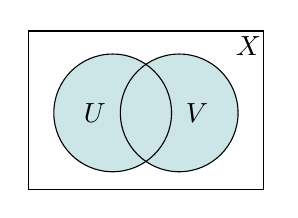
\begin{tikzpicture}[scale=.65]
\draw (-2.3,-1.5) rectangle (2.3,1.6);
\fill[ProofTeal!20] (-.65,0) circle(1.15);
\fill[ProofTeal!20] (.65,0) circle(1.15);
\draw (-.65,0) circle(1.15); \draw (.65,0) circle(1.15);
\node at (-1,0) {$U$}; \node at (1,0) {$V$}; \node at (2,1.3) {$X$};
\end{tikzpicture}
\[
 U\cup V
\]
To prove membership, establish at least one side.
From membership, be ready for two cases.
\end{column}
\begin{column}{.49\textwidth}
\centering
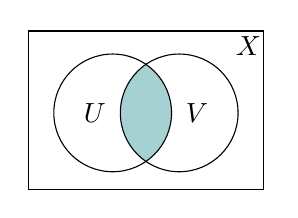
\begin{tikzpicture}[scale=.65]
\draw (-2.3,-1.5) rectangle (2.3,1.6);
\begin{scope}
\clip (-.65,0) circle(1.15);
\fill[ProofTeal!35] (.65,0) circle(1.15);
\end{scope}
\draw (-.65,0) circle(1.15); \draw (.65,0) circle(1.15);
\node at (-1,0) {$U$}; \node at (1,0) {$V$}; \node at (2,1.3) {$X$};
\end{tikzpicture}
\[
 U\cap V
\]
To prove membership, establish both sides.
From membership, obtain two usable facts.
\end{column}
\end{columns}
\sourcecredit{Examples 9.2.1 and 9.2.3; original diagrams}
\end{frame}

% Source: Example 9.2.3.
% Correction: its prose says real numbers, but both statement and Lean use Q.
\begin{frame}{A worked intersection proof uses both hypotheses}
\textbf{Claim.}
\[
 \{-2,3\}\cap\{x:\Q\mid x^2=9\}\subseteq\{x:\Q\mid0<x\}.
\]
\textbf{Proof.} Fix $t\in\Q$ in the intersection. Then
\[
 (t=-2\ \lor\ t=3)\qquad\text{and}\qquad t^2=9.
\]
\begin{itemize}
\item If $t=-2$, then $t^2=4$. Together with $t^2=9$, this gives $4=9$, a contradiction.
\item If $t=3$, then $0<t$.
\end{itemize}
The first condition narrows the possibilities; the second rules out the unwanted one.
Thus every element of the intersection is positive.
\sourcecredit{Example 9.2.3}
\end{frame}

% Source: Examples 9.2.6--9.2.7.
% Correction: 9.2.6's prose repeats residue 1 and changes Z to N; the Lean statement
% uses two sets in Z, residues 1 and 2 modulo 5, as used here.
\begin{frame}{Empty sets and universal sets require different proofs}
\textbf{An empty intersection.} Let
$A=\{n:\Z\mid n\equiv1\pmod5\}$ and
$B=\{n:\Z\mid n\equiv2\pmod5\}$.
If $x\in A\cap B$, then $x=1+5k=2+5l$ for some integers $k,l$.
Thus $1=5(k-l)$, impossible. Hence $A\cap B=\emptyset$.
\medskip

\textbf{A universal union.} Let $C=\{x:\R\mid-1<x\}$ and
$D=\{x:\R\mid x<1\}$. For an arbitrary $t\in\R$:
\begin{itemize}
\item if $t\le0$, then $t<1$, so $t\in D$;
\item if $t>0$, then $-1<t$, so $t\in C$.
\end{itemize}
Therefore every real number belongs to $C\cup D$, and $C\cup D=\R$.
\sourcecredit{Examples 9.2.6--9.2.7}
\end{frame}

% Source: Example 9.2.2 and explicit-set tactic in Exercises 9.2.8.
\begin{frame}[fragile]{Lean: Arithmetic facts versus propositional structure}
\begin{lstlisting}
example : Set.union ({1, 2} : Set Nat) {2, 4}
    = {1, 2, 4} := by
  ext n
  dsimp
  exhaust
\end{lstlisting}
After unfolding, the goal is the logical equivalence
\[
 ((n=1\lor n=2)\lor(n=2\lor n=4))
 \ \Longleftrightarrow\ (n=1\lor n=2\lor n=4).
\]
The book's \texttt{exhaust} handles this propositional rearrangement.
It does not replace a needed arithmetic argument such as proving two residue conditions incompatible.
\medskip

For an intersection hypothesis, split the conjunction; for a union hypothesis,
split into cases. These are the same proof patterns used before sets were introduced.
\sourcecredit{Example 9.2.2; Exercises 9.2.8}
\end{frame}

% Source: Explicit intersection/complement exercises in 9.2.8.
% The De Morgan identity is an original transfer exercise using the same definitions.
\begin{frame}{Practice 9.2: Calculate, then prove a general identity}
\begin{enumerate}
\item In the ambient type $\N$, simplify
\[
 \{0,1,2,3,4\}\cap\{0,2,4,6,8\},\qquad
 \{3,4,5\}^c\cap\{1,3,5,7,9\}.
\]
\item For arbitrary sets $U,V$ in the same type $X$, prove
\[
 (U\cup V)^c=U^c\cap V^c.
\]
Start with an arbitrary $x\in X$ and translate each side into logic.
\end{enumerate}
The picture can suggest an answer. A membership proof establishes it for every element.
\sourcecredit{Exercises 9.2.8; original general-identity exercise}
\end{frame}

% Source: New solutions; De Morgan proof is original.
\begin{frame}{Practice 9.2: Solution ideas}
The explicit intersections are $\{0,2,4\}$ and $\{1,7,9\}$.
In the second expression, remove $3$ and $5$ from the listed set; $4$ was absent already.
\medskip

For the identity, fix $x\in X$.
\begin{itemize}
\item Suppose $x\notin U\cup V$. If $x\in U$, it would belong to the union;
similarly for $V$. Hence $x\notin U$ and $x\notin V$, so $x\in U^c\cap V^c$.
\item Suppose $x\in U^c\cap V^c$. Then $x\notin U$ and $x\notin V$.
Either case of $x\in U\cup V$ contradicts one of these facts.
Thus $x\notin U\cup V$.
\end{itemize}
The membership conditions are equivalent for every $x$, so extensionality gives the set equality.
\sourcecredit{Section 9.2 definitions; solutions to the preceding practice}
\end{frame}

\section{9.3 The type of sets}
% Source: Definition 9.3.1 and Example 9.3.2.
\begin{frame}{9.3: A set can itself be an element}
The type of all sets in $X$ is written $\mathcal P(X)$ on paper and \texttt{Set X} in Lean.
\begin{center}
\begin{tabular}{ll}
\toprule
Object & Type\\\midrule
$3$ & $\N$\\
$\{3,4\}$ & $\mathcal P(\N)$\\
$\{\{3,4\},\{4,5,6\}\}$ & $\mathcal P(\mathcal P(\N))$\\
$\mathcal F=\{S:\mathcal P(\N)\mid3\in S\}$ & $\mathcal P(\mathcal P(\N))$\\
\bottomrule
\end{tabular}
\end{center}
For the set $E$ of even natural numbers, $E\notin\mathcal F$ because $3\notin E$.
However, $\{3,4\}\in\mathcal F$ because $3\in\{3,4\}$.
\medskip

Membership $S\in\mathcal F$ and inclusion $S\subseteq T$ are different statements about different types.
\sourcecredit{Definition 9.3.1; Example 9.3.2}
\end{frame}

% Source: Example 9.3.3; original explanation of the information lost at zero.
\begin{frame}{A function on sets can lose information}
Define $p:\mathcal P(\N)\to\mathcal P(\N)$ by
\[
 p(S)=\{n:\N\mid n+1\in S\}.
\]
For instance, $p(\{0,2,4\})=\{1,3\}$.
\begin{block}{Claim: $p$ is not injective}
Take $S=\{0\}$ and $T=\emptyset$.
Since $n+1>0$ for every $n\in\N$, no $n$ satisfies $n+1\in S$.
Thus $p(S)=\emptyset=p(T)$.
But $S\ne T$, because $0\in S$ and $0\notin T$.
\end{block}
The output never tests whether $0\in S$; all tested inputs have the form $n+1$.
\sourcecredit{Example 9.3.3}
\end{frame}

% Source: Example 9.3.4, with the k-1 test written explicitly.
\begin{frame}{The same rule over integers preserves information}
Define $q:\mathcal P(\Z)\to\mathcal P(\Z)$ by
$q(S)=\{n:\Z\mid n+1\in S\}$.
\medskip

\textbf{Claim.} $q$ is injective.
Suppose $q(S)=q(T)$. To prove $S=T$, fix an arbitrary $k\in\Z$.
Then $k-1$ is also an integer, and
\[
\begin{aligned}
 k\in S
 &\iff (k-1)+1\in S\\
 &\iff k-1\in q(S)\\
 &\iff k-1\in q(T)\\
 &\iff (k-1)+1\in T\\
 &\iff k\in T.
\end{aligned}
\]
Extensionality gives $S=T$. The ability to use $k-1$ is essential.
\sourcecredit{Example 9.3.4}
\end{frame}

% Source: Example 9.3.5; original finite membership matrix illustration.
\begin{frame}{Cantor's construction: A set that differs on the diagonal}
\begin{block}{Theorem}
For every type $X$, no function $f:X\to\mathcal P(X)$ is surjective.
\end{block}
Define $D=\{x:X\mid x\notin f(x)\}$.
The membership of $x$ in $D$ is the opposite of its membership in $f(x)$.
\begin{columns}[T]
\begin{column}{.45\textwidth}
\centering
\begin{tabular}{c|cccc}
 & $a$ & $b$ & $c$ & $d$\\\hline
$f(a)$ & \textbf{1} & 0 & 1 & 0\\
$f(b)$ & 1 & \textbf{0} & 0 & 1\\
$f(c)$ & 0 & 1 & \textbf{1} & 1\\
$f(d)$ & 1 & 0 & 0 & \textbf{0}\\\hline
$D$ & 0 & 1 & 0 & 1
\end{tabular}
\end{column}
\begin{column}{.51\textwidth}
In this illustrative finite table, $1$ means membership and $0$ means nonmembership.
\medskip

$D$ differs from row $f(a)$ at column $a$, from row $f(b)$ at column $b$, and so on.
The definition works without enumerating $X$.
\end{column}
\end{columns}
\sourcecredit{Example 9.3.5; original membership matrix}
\end{frame}

% Source: Example 9.3.5; complete diagonal argument, phrased without the barber story.
\begin{frame}{Cantor's proof: The proposed preimage contradicts itself}
Assume $f:X\to\mathcal P(X)$ is surjective and set
$D=\{x:X\mid x\notin f(x)\}$.
Surjectivity supplies $d\in X$ with $f(d)=D$. Consequently,
\[
 d\in D\quad\Longleftrightarrow\quad d\notin f(d)
 \quad\Longleftrightarrow\quad d\notin D.
\]
\begin{itemize}
\item If $d\in D$, the defining condition gives $d\notin f(d)=D$, a contradiction.
\item If $d\notin D$, then $d\notin f(d)$ because $f(d)=D$.
By the definition of $D$, this says $d\in D$, again a contradiction.
\end{itemize}
Thus the assumption of surjectivity is impossible.
\medskip

The obstruction applies to every proposed function $f$; the diagonal set is built from that very function.
\sourcecredit{Example 9.3.5}
\end{frame}

% Source: Example 9.3.5, adapted to ASCII predicates and cases syntax.
% Set application (f x) x is definitionally the membership x in f x.
\begin{frame}[fragile]{Lean: The diagonal set is a predicate}
\begin{lstlisting}
example {X : Type} (f : X -> Set X) : Not (Function.Surjective f) := by
  intro hf
  let D : Set X := fun x => Not ((f x) x)
  cases hf D with
  | intro d hd =>
      by_cases h : D d
      case pos =>
        have hn : Not ((f d) d) := h
        rw [hd] at hn
        exact hn h
      case neg =>
        have hn : Not (Not ((f d) d)) := h
        rw [hd] at hn
        exact hn h
\end{lstlisting}
Here \texttt{D d} means $d\in D$, since a set is represented by a predicate.
\sourcecredit{Example 9.3.5; textbook-environment demonstration}
\end{frame}

% Source: Both Exercises 9.3.6.
\begin{frame}{Practice 9.3: Sets as function values and sequence terms}
\begin{enumerate}
\item Define $r:\mathcal P(\N)\to\mathcal P(\N)$ by $r(S)=S\cup\{3\}$.
Prove that $r$ is not injective.
\item Define a sequence of sets of integers by
\[
 U_0=\Z,\qquad
 U_{n+1}=\{x:\Z\mid\exists y\in U_n,\ x=2y\}.
\]
Prove by induction that $U_n=\{x:\Z\mid2^n\mid x\}$ for every $n\in\N$.
\end{enumerate}
In the second task, the induction hypothesis is an equality of sets.
Use it to replace a membership condition, then translate divisibility into a witness equation.
\sourcecredit{Exercises 9.3.6}
\end{frame}

% Source: Newly written solutions to Exercises 9.3.6.
\begin{frame}{Practice 9.3: Solution ideas}
\textbf{The union function.} The distinct inputs $\emptyset$ and $\{3\}$ both map to
$\{3\}$. They are distinct because only the second contains $3$.
\medskip

\textbf{The sequence.} For $n=0$, $2^0=1$ divides every integer, so the formula gives $U_0=\Z$.
Assume the formula for $U_n$ and fix $x\in\Z$.
\begin{itemize}
\item If $x\in U_{n+1}$, write $x=2y$ with $y\in U_n$.
The induction hypothesis gives $y=2^n k$ for some $k\in\Z$.
Then $x=2^{n+1}k$.
\item If $x=2^{n+1}k$, set $y=2^n k$.
Then $y\in U_n$ by the induction hypothesis and $x=2y$, so $x\in U_{n+1}$.
\end{itemize}
These implications prove the required set equality at $n+1$.
\sourcecredit{Exercises 9.3.6}
\end{frame}

% Source: Review synthesized from Sections 9.1--9.3.
\begin{frame}{Chapter 9 review: Expose the underlying logic}
\begin{center}
\begin{tabular}{p{.30\textwidth}p{.56\textwidth}}
\toprule
Set statement & Proof obligation\\\midrule
$x\in\{t\mid P(t)\}$ & Prove $P(x)$.\\
$U\subseteq V$ & Start with arbitrary $x\in U$; prove $x\in V$.\\
$U=V$ & Prove both directions of membership.\\
$U\ne V$ & Find an element in exactly one set.\\
$U=\emptyset$ & Rule out an arbitrary proposed member.\\
$U=\operatorname{univ}_X$ & Show every $x\in X$ belongs.\\
$S\in\mathcal F$ & Apply the family's predicate to the set $S$.\\
\bottomrule
\end{tabular}
\end{center}
\textbf{Exit check.} For $\mathcal F=\{S:\mathcal P(\N)\mid0\in S\}$,
explain why $\{0\}\in\mathcal F$ is well-typed and why $0\in\mathcal F$ is not.
\sourcecredit{Sections 9.1--9.3}
\end{frame}

% Source and adaptation statement for the chapter.
\begin{frame}{Reading and code context}
Heather Macbeth, \emph{The Mechanics of Proof}, Chapter 9:
\begin{itemize}
\item 9.1 Introduction
\item 9.2 Set operations
\item 9.3 The type of sets
\end{itemize}
\url{https://hrmacbeth.github.io/math2001/09_Sets.html}
\medskip

These notes use original explanations, diagrams, and practice solutions around the cited material.
Lean examples use the textbook's teaching environment. In ASCII listings,
\texttt{Set.Subset} names inclusion, \texttt{Set.union} names union, and
\texttt{Exists} introduces an existential predicate.
\end{frame}
\end{document}
